\documentclass[../../General.tex]{subfiles}
\begin{document}


\section{Estado del arte} 

\subsection{Soluciones integrales}
En esta sección se analizan los sistemas mecatrónicos completos que intentan resolver el problema general de la inspección y medición dentro de los parques solares fotovoltaicos, sirviendo como referentes de diseño global para el vehículo terrestre autónomo propuesto.

\subsubsection{\textbf{Estación meteorológica fotovoltaica móvil (CN 216956405 U):}} Esta patente describe, como se ilustra en la Figura \ref{fig:CN216956405U} (izquierda), una estación climática (2) montada sobre una base con ruedas, vista en Figura la \ref{fig:CN216956405U} (derecha), que incluye soportes roscados, compuestos por una funda roscada y una varilla roscada, y placas o almohadillas estabilizadoras (5) que se despliegan hacia abajo para anclar el equipo en superficies desniveladas. El sistema destaca por su enfoque en la estabilización mecánica del equipo de medición, utilizando estos mecanismos de anclaje desplegables que aseguran que los sensores meteorológicos mantengan un plano de referencia adecuado al evitar que la base se incline, así como evita volcaduras el recorrido en terrenos con pendiente.
	
	\begin{figure}[H]
		
		\captionsetup{justification=raggedright, singlelinecheck=false, labelsep=none}
		
		\caption[Ilustraciones de estación meteorológica fotovoltaica móvil.]{} 
		
		\textit{Ilustraciones de estación meteorológica fotovoltaica móvil.} \par\medskip
		
		\begin{minipage}{0.4\textwidth}
			\centering
			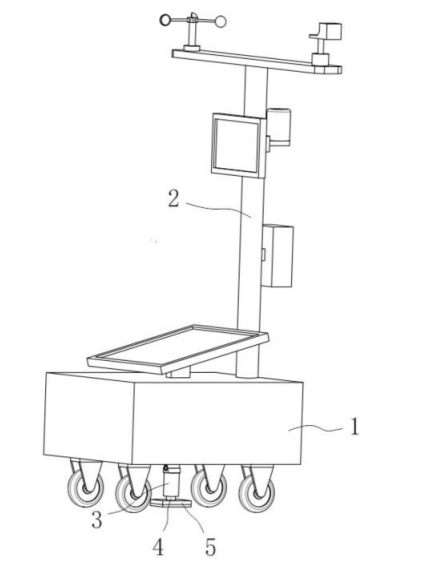
\includegraphics[width=\linewidth]{Recursos/Imagenes/ImagenesEstadoDelArte/CN216956405U-1.png}
		\end{minipage}\hfill
		\begin{minipage}{0.4\textwidth}
			\centering
			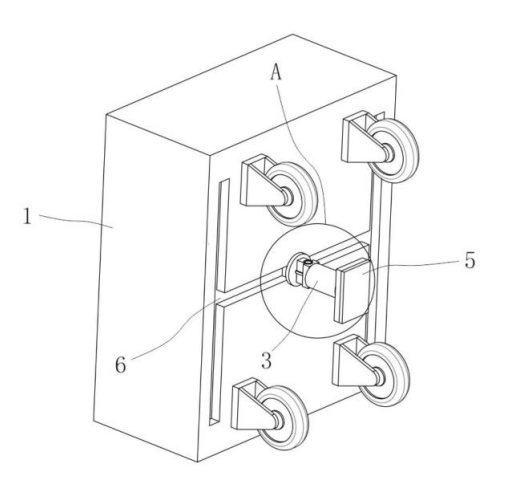
\includegraphics[width=\linewidth]{Recursos/Imagenes/ImagenesEstadoDelArte/CN216956405U-2.png}
		\end{minipage}
		\par\medskip
		
		\raggedright
		\footnotesize \textit{Nota.} Adaptado de \cite{CN216956405U}.
		\label{fig:CN216956405U}
	\end{figure}
	
	
\subsubsection{\textbf{Vehículo de inspección para plantas de energía fotovoltaicas (CN 218409341 U):}} Es un vehículo terrestre no tripulado, mostrado en la Figura \ref{fig:CN218409341U}, montado sobre una base (1), equipado con ruedas de movimiento (21), paneles solares abatibles (12) para carga y un robusto mecanismo de amortiguación mediante resortes (20) en cajas para evitar daños en la instrumentación durante el tránsito. Esta patente representa una solución integral para la problemática, implementando el uso de paneles solares integrados para la recarga autónoma y sistemas de amortiguación para la protección de la instrumentación, lo que asegura la precisión de las mediciones dinámicas y prolonga la autonomía.
	
	\begin{figure}[H]
		\captionsetup{justification=raggedright, singlelinecheck=false, labelsep=none}
		
		\caption[Ilustración de vehículo de inspección con paneles solares y sistema de amortiguación.]{} 
		
		\textit{Ilustración de vehículo de inspección terrestre con paneles solares abatibles y mecanismo de amortiguación.} \par\medskip
		
		\centering
		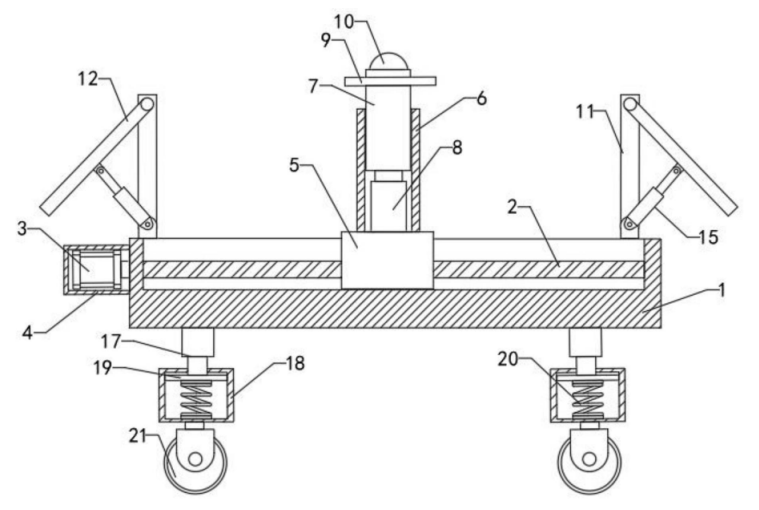
\includegraphics[width=0.75\textwidth]{Recursos/Imagenes/ImagenesEstadoDelArte/CN218409341U.png} \par\medskip
		
		\raggedright
		\footnotesize \textit{Nota.} Adaptado de \cite{CN218409341U}.
		\label{fig:CN218409341U}
	\end{figure}
\subsubsection{\textbf{Vehículo de inspección para plantas fotovoltaicas en desiertos (CN 221163061 U):}} 
Este robot, como se ilustra en la Figura \ref{fig:CN221163061U}, cuenta con tracción de orugas (2) diseñada con ángulos de inclinación anti-deslizamiento (22) y está equipado con radar y sensores de viento, humedad y radiación o luz. La propuesta se alinea con el propósito general del proyecto, ya que el diseño integrado de un tren de tracción para terrenos desérticos acoplado a un sistema completo de sensores climáticos sirve como el principal punto de referencia comercial y tecnológico para validar la arquitectura y el alcance funcional del UGV de irradiancia propuesto.
	
	\begin{figure}[H]
		\captionsetup{justification=raggedright, singlelinecheck=false, labelsep=none}
		
		\caption[Ilustración de robot de inspección para estaciones fotovoltaicas en el desierto.]{} 
		
		\textit{Ilustración de robot de inspección con tracción de orugas y sensores climáticos para entornos desérticos.} \par\medskip
		
		\centering
		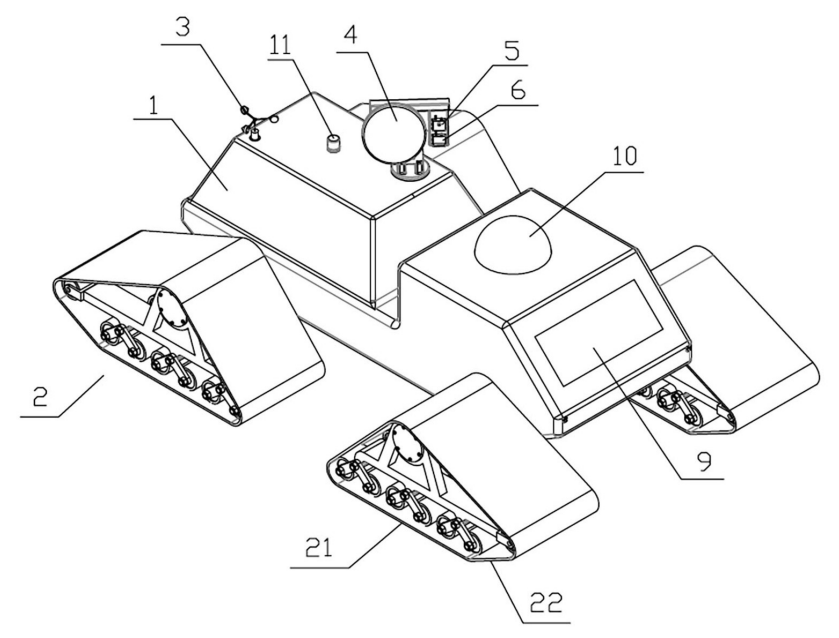
\includegraphics[width=0.7\textwidth]{Recursos/Imagenes/ImagenesEstadoDelArte/CN221163061U.png} \par\medskip
		
		\raggedright
		\footnotesize \textit{Nota.} Adaptado de \citep{CN221163061U}.
		\label{fig:CN221163061U}
	\end{figure}
%%
%%
\begin{center}
\footnotesize
\begin{xltabular}{\textwidth}{|p{2.5cm}|>{\raggedright\arraybackslash}X|>{\raggedright\arraybackslash}X|>{\raggedright\arraybackslash}X|}
\caption{Análisis comparativo de Soluciones Integrales.}
\label{tab:estado_arte_integrales} \\
\hline
\rowcolor[HTML]{D9E1F2} 
\textbf{Referente} & \textbf{Principio de Funcionamiento} & \textbf{Aporte al Proyecto} & \textbf{Limitaciones} \\ \hline
\endfirsthead

\multicolumn{4}{c}%
{{\bfseries Continuación de la \tablename\ \thetable{}}} \\
\hline
\rowcolor[HTML]{D9E1F2} 
\textbf{Referente} & \textbf{Principio de Funcionamiento} & \textbf{Aporte al Proyecto} & \textbf{Limitaciones} \\ \hline
\endhead

\hline
\endfoot

\hline
\endlastfoot

%%
%%
%%

Estación meteorológica fotovoltaica móvil (CN 216956405 U)  & Estación sobre ruedas que emplea soportes roscados y almohadillas estabilizadoras de despliegue mecánico. & Proporciona mecanismos de nivelación y estabilización para asegurar el plano horizontal durante la lectura estática de sensores. & Tracción por ruedas ineficiente en terrenos irregulares; la nivelación pausada ralentiza el proceso de inspección dinámica. \\ \hline

Vehículo de inspección para plantas de energía fotovoltaicas (CN 218409341 U)  & Vehículo terrestre (UGV) con paneles solares abatibles y un mecanismo robusto de amortiguación con resortes en cajas. & Extiende la autonomía energética del robot e incorpora suspensión vital para proteger instrumentos sensibles de las vibraciones. & Locomoción por ruedas; carece de actuadores o mecanismos para limpiar los instrumentos ante la acumulación de polvo. \\ \hline

Vehículo de inspección para plantas fotovoltaicas en desiertos (CN 221163061 U)  & Chasis hermético propulsado por orugas antideslizantes, equipado con radar y sensores de radiación, viento y humedad. & Modelo de arquitectura mecatrónica base para un UGV desértico, combinando alta movilidad con medición climatológica. & Instrumentación estática en el chasis; no cuenta con ejes para adaptar la elevación o inclinación de los sensores a los paneles. \\ \hline

\end{xltabular}
\end{center}

%%
%%
\vspace{-1.5cm}
%%
\subsection{Soluciones parciales}
En esta sección se describen los componentes y subsistemas especializados que abordan necesidades técnicas específicas, clasificados según su funcionalidad.

\subsubsection{Robots para plantas fotovoltaicas}
\begin{itemize}
	\item \textbf{Vehículo de inspección terrestre inteligente para plantas fotovoltaicas (CN 119665962 A):} Esta patente, ilustrada en la Figura \ref{fig:CN119665962A&CN120057153A} (izquierda), describe un vehículo terrestre no tripulado cuya base (10) que incorpora soportes (20) y una carcasa superior (40) que aloja un panel fotovoltaico (30). Este vehículo está diseñado para la generación de mapas espaciales y la planificación de rutas globales de forma autónoma. El sistema integra algoritmos de navegación y percepción que le permiten realizar la recolección de datos ambientales en movimiento y la evasión de obstáculos en el terreno de manera autónoma.
	
	\item \textbf{Robot de inspección de alta transitabilidad para plantas fotovoltaicas (CN 120057153 A):} Ilustrado en la Figura \ref{fig:CN119665962A&CN120057153A} (derecha), se trata de un vehículo con tracción mediante ruedas activas (31) (con opción de incluir configuraciones de oruga) conectadas a módulos flotantes (32) de amortiguación con resortes oscilantes (35). Este diseño está concebido para operar en entornos con topografía irregular, como suelo desértico o con pendientes pronunciadas. Su configuración mecánica también incluye un brazo base (4) desplegable desde un compartimento de almacenamiento (2) para labores de inspección, el cual garantiza la estabilidad y movilidad del robot frente a obstáculos comunes en las plantas solares a gran escala, permitiéndole navegar entre los paneles incluso cuando la distancia al suelo es reducida.
	
	
	\begin{figure}[H]
		
		\captionsetup{justification=raggedright, singlelinecheck=false, labelsep=none}
		
		\caption[Ilustraciones de vehículo de inspección terrestre inteligente y robot de inspección de alta transitabilidad.]{} 
		
		\textit{Ilustraciones de vehículo de inspección terrestre inteligente y robot de inspección de alta transitabilidad.} \par\medskip
		
		\begin{minipage}{0.6\textwidth}
			\centering
			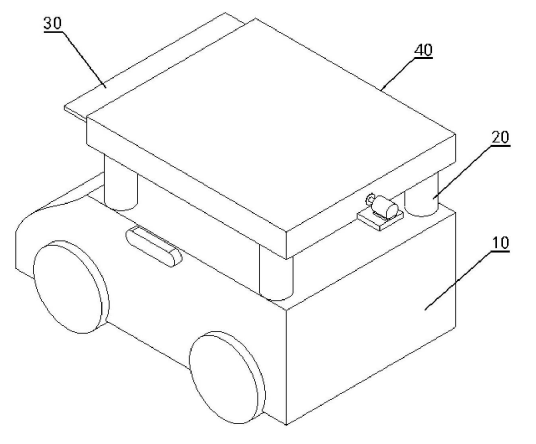
\includegraphics[width=\linewidth]{Recursos/Imagenes/ImagenesEstadoDelArte/CN119665962A.png}
		\end{minipage}\hfill
		\begin{minipage}{0.5\textwidth}
			\centering
			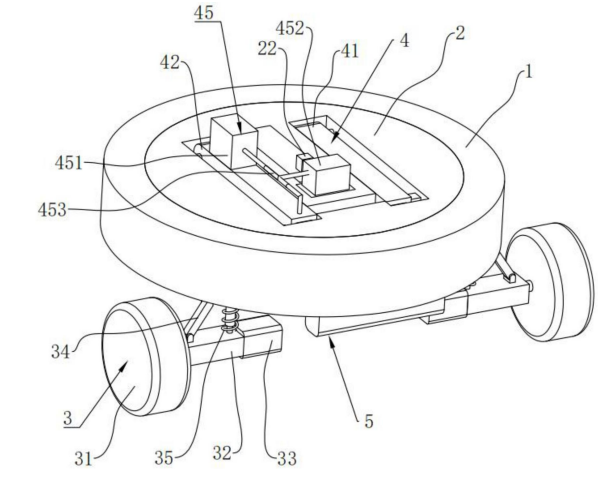
\includegraphics[width=\linewidth]{Recursos/Imagenes/ImagenesEstadoDelArte/CN120057153A.png}
		\end{minipage}
		\par\medskip
		
		\raggedright
		\footnotesize \textit{Nota.} Adaptado de \cite{CN119665962A} (izquierda) y \cite{CN120057153A} (derecha).
		\label{fig:CN119665962A&CN120057153A}
	\end{figure}
	
	\item \textbf{Dispositivo de inspección automática para plantas fotovoltaicas (CN 220873036 U):} Este robot móvil, ilustrado en la Figura \ref{fig:CN220873036U}, comprende un cuerpo (1) sobre un mecanismo de desplazamiento, destaca por incorporar un motor (17) y un brazo giratorio o varilla (18) equipado con un cepillo o esponja (19) automatizado para la limpieza de los lentes de sus cámaras y mecanismos de captura de imágenes (8). Esta solución mecatrónica es esencial para mitigar el impacto del \textit{soiling} en los propios instrumentos del vehículo, como la plataforma de imágenes infrarrojas, asegurando la correcta lectura en las mediciones meteorológicas durante operaciones prolongadas en entornos con mucho polvo.
	
	\begin{figure}[H]
		\captionsetup{justification=raggedright, singlelinecheck=false, labelsep=none}
		
		\caption[Ilustración de vehículo de inspección con sistema de limpieza de sensores]{} 
		
		\textit{Ilustración de dispositivo de inspección automática con mecanismos de limpieza para sus instrumentos ópticos.} \par\medskip
		
		\centering
		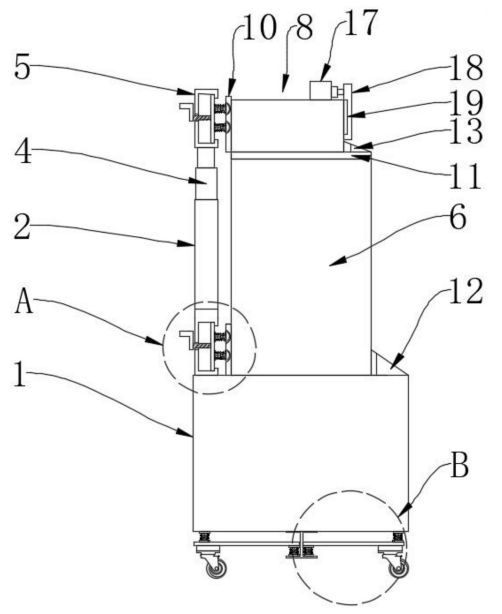
\includegraphics[width=0.4\textwidth]{Recursos/Imagenes/ImagenesEstadoDelArte/CN220873036U.png} \par\medskip
		
		\raggedright
		\footnotesize \textit{Nota.} Adaptado de \cite{CN220873036U}.
		\label{fig:CN220873036U}
	\end{figure}
\end{itemize}

\begin{table}[H]
	\centering
	\footnotesize
	\caption{Análisis comparativo de Soluciones Parciales: Robots para plantas fotovoltaicas.}
	\label{tab:estado_arte_robots_pv}
	\begin{tabularx}{\textwidth}{|p{3.5cm}|>{\raggedright\arraybackslash}X|>{\raggedright\arraybackslash}X|>{\raggedright\arraybackslash}X|}
		\hline
		\rowcolor[HTML]{D9E1F2} 
		\textbf{Referente} & \textbf{Principio de Funcionamiento} & \textbf{Aporte al Proyecto} & \textbf{Limitaciones} \\ \hline
		Vehículo de inspección terrestre inteligente para plantas fotovoltaicas (CN 119665962 A) & Emplea algoritmos de control y datos ambientales para generar mapas espaciales y trazar rutas. & Aporta la arquitectura lógica para la navegación autónoma global y la evasión dinámica de obstáculos en la planta. & Cubre únicamente el dominio de software y control; no soluciona los retos mecánicos de tracción ni de captura física de datos. \\ \hline
		Robot de inspección de alta transitabilidad para plantas fotovoltaicas (CN 120057153 A) & Tren de locomoción basado en orugas acoplado a módulos flotantes de amortiguación para mantener el equilibrio. & Diseño mecánico ideal para sortear terrenos muy complejos, zanjas erosivas y pendientes de arena suelta. & Enfoque puramente cinemático y estructural; no integra sistemas de comunicación o instrumentación meteorológica. \\ \hline
		Dispositivo de inspección automática para plantas fotovoltaicas (CN 220873036 U) & Brazo robótico automatizado equipado con esponja o cepillo para frotar y limpiar los lentes de a bordo. & Estrategia de interacción física para mitigar de forma activa el soiling en los instrumentos durante largos recorridos. & Sistema optimizado para cámaras frontales; requiere rediseño para no dañar los domos de vidrio de los piranómetros. \\ \hline
	\end{tabularx}
\end{table}

\subsubsection{Robots para inspección de plantas de energía}
\begin{itemize}
	\item \textbf{Robot de inspección inteligente para plantas de energía (CN 215511023 U):} Esta plataforma móvil de orugas, como se ilustra en la Figura \ref{fig:CN215511023U&CN215701759U} (izquierda), integra un brazo mecánico (4) y un sistema de visión compuesto por una cámara óptica y un sensor infrarrojo. Una característica innovadora de este diseño es la inclusión de un sensor de nivel de líquidos (8) en su parte inferior, lo que permite al vehículo detectar y evadir charcos de lodo o zonas inundadas para proteger la integridad de sus componentes electrónicos, como el host de control central (7).
	
	\item \textbf{Robot de inspección para plantas de energía con mecanismo de corte (CN 215701759 U):} Este vehículo, como se ilustra en la Figura \ref{fig:CN215511023U&CN215701759U} (derecha) está equipado con un brazo giratorio (7) que posee un motor (8) y aspas de corte integradas (9). Este mecanismo permite al robot abrirse paso a través de vegetación o maleza que pueda obstruir las rutas de inspección, garantizando la continuidad del servicio de mantenimiento.
	
	
		\begin{figure}[H]
		
		\captionsetup{justification=raggedright, singlelinecheck=false, labelsep=none}
		
		\caption[Ilustraciones de robot de inspección con sensor de líquidos y robot de inspección con mecanismo de corte de maleza.]{} 
		
		\textit{Ilustraciones de robot de inspección con sensor de líquidos y robot de inspección con mecanismo de corte de maleza.} \par\medskip
		
		\begin{minipage}{0.5\textwidth}
			\centering
			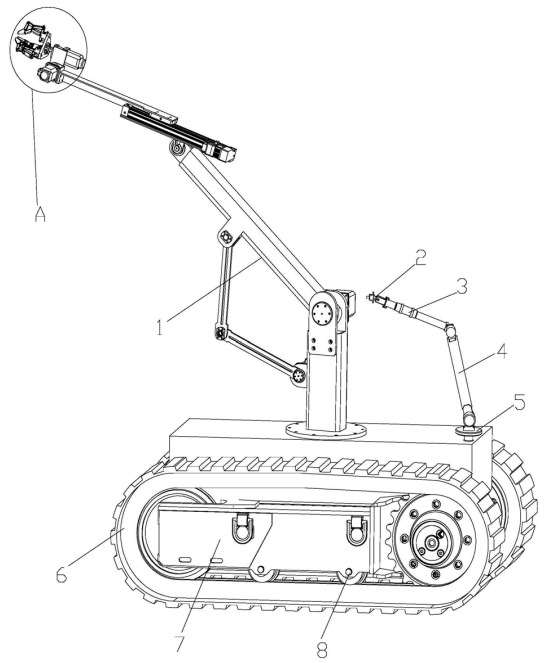
\includegraphics[width=\linewidth]{Recursos/Imagenes/ImagenesEstadoDelArte/CN215511023U.png}
		\end{minipage}\hfill
		\begin{minipage}{0.6\textwidth}
			\centering
			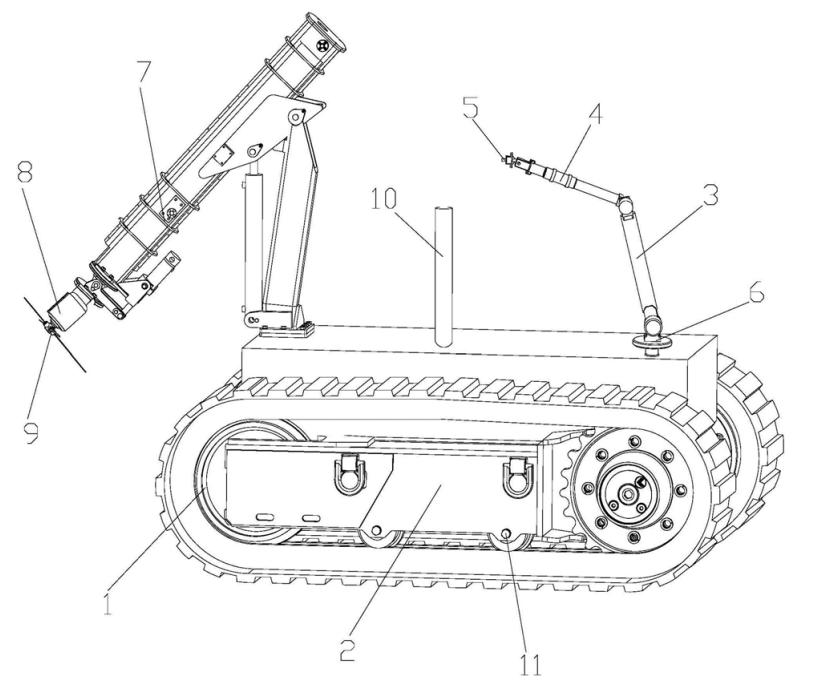
\includegraphics[width=\linewidth]{Recursos/Imagenes/ImagenesEstadoDelArte/CN215701759U.png}
		\end{minipage}
		\par\medskip
		
		\raggedright
		\footnotesize \textit{Nota.} Adaptado de \cite{CN215511023U} (izquierda) y \cite{CN215701759U} (derecha).
		\label{fig:CN215511023U&CN215701759U}
	\end{figure}
	
	
	
\end{itemize}
%%%%%%

\begin{table}[H]
	\centering
	\footnotesize
	\caption{Análisis comparativo de Soluciones Parciales: Robots para inspección en general.}
	\label{tab:estado_arte_robots_general}
	\begin{tabularx}{\textwidth}{|p{3.5cm}|>{\raggedright\arraybackslash}X|>{\raggedright\arraybackslash}X|>{\raggedright\arraybackslash}X|}
		\hline
		\rowcolor[HTML]{D9E1F2} 
		\textbf{Referente} & \textbf{Principio de Funcionamiento} & \textbf{Aporte al Proyecto} & \textbf{Limitaciones} \\ \hline
		Robot de inspección inteligente para plantas de energía (CN 215511023 U) & Dispone de un sensor de nivel de líquidos en el tren inferior para detectar acumulación de agua. & Mecanismo de seguridad que funciona como alarma para evadir charcos de lodo, protegiendo la electrónica inferior. & Medida preventiva que detiene el avance; ante zonas altamente inundadas, el robot perdería su ruta planificada. \\ \hline
		Robot de inspección para plantas de energía con mecanismo de corte (CN 215701759 U) & Integra un brazo telescópico giratorio equipado con aspas de corte accionadas por motor eléctrico. & Brinda una solución mecánica para abrir paso en pasillos bloqueados por crecimiento de vegetación alta o maleza. & Alto consumo energético para la batería; aumenta la complejidad y el peso estructural frontal del vehículo. \\ \hline
	\end{tabularx}
\end{table}

\subsubsection{Estaciones meteorológicas para plantas fotovoltaicas}
\begin{itemize}
\item \textbf{Estación meteorológica solar multi-elemento (CN 216243088 U):} Esta estación meteorológica, como se ilustra en la Figura \ref{fig:CN216243088U&CN206638837U} (izquierda), emplea un trípode adaptativo (1) equipado con placas de refuerzo (3) y anclajes de fijación (14) con mecanismos de resorte. Este diseño, que soporta la caja meteorológica principal (11) y el panel solar (13), permite proporcionar una fijación mecánica rígida y estabilidad temporal a la estructura frente a ráfagas de viento fuertes, evitando que las vibraciones afecten la precisión de las mediciones ambientales.


\item \textbf{Sistema de monitoreo de estación meteorológica para módulos fotovoltaicos (CN 206638837 U):} El sistema, como se ilustra en la Figura \ref{fig:CN216243088U&CN206638837U} (derecha), propone una estructura con rieles y soportes móviles ,tales como la sección de colocación (1), que permiten ajustar la posición y el ángulo de los sensores y paneles solares (13). Esta funcionalidad facilita la alineación precisa de la instrumentación con el ángulo de las celdas solares fijas o dinámicas, permitiendo realizar mediciones exactas en el plano del panel fotovoltaico.




\begin{figure}[H]
	
	\captionsetup{justification=raggedright, singlelinecheck=false, labelsep=none}
	
	\caption[Ilustraciones de estación meteorológica con trípode adaptativo y estructura de soporte móvil con alineación.]{} 
	
	\textit{Ilustraciones de estación meteorológica con trípode adaptativo y estructura de soporte móvil con alineación.} \par\medskip
	
	\begin{minipage}{0.5\textwidth}
		\centering
		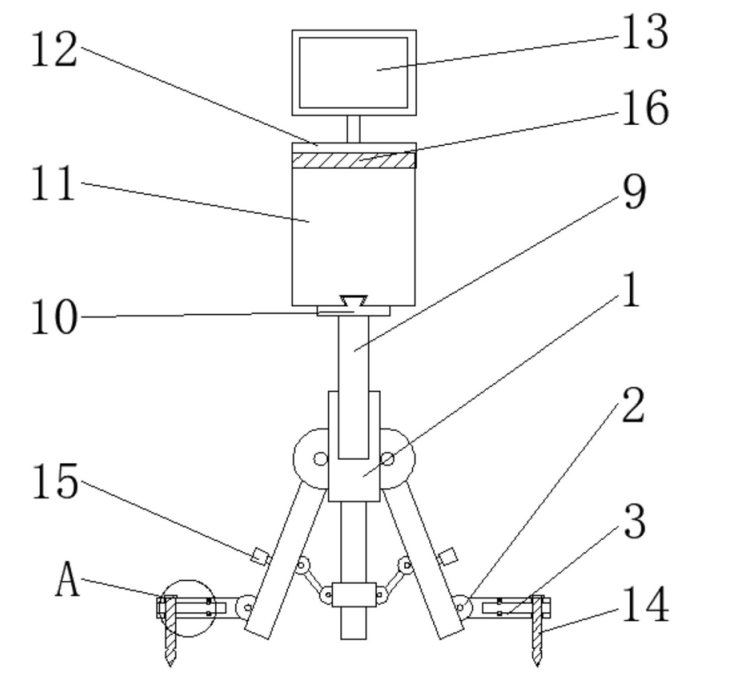
\includegraphics[width=\linewidth]{Recursos/Imagenes/ImagenesEstadoDelArte/CN216243088U.png}
	\end{minipage}\hfill
	\begin{minipage}{0.5\textwidth}
		\centering
		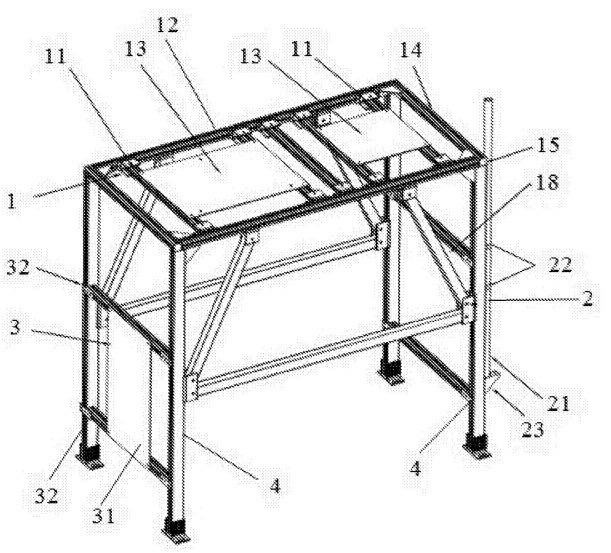
\includegraphics[width=\linewidth]{Recursos/Imagenes/ImagenesEstadoDelArte/CN206638837U.png}
	\end{minipage}
	\par\medskip
	
	\raggedright
	\footnotesize \textit{Nota.} Adaptado de \cite{CN216243088U} (izquierda) y \cite{CN206638837U} (derecha).
	\label{fig:CN216243088U&CN206638837U}
\end{figure}

\item \textbf{Estación meteorológica simple para monitoreo ambiental (CN 206362955 U):} Se describe, como se ilustra en la Figura \ref{fig:CN206362955U&CN222047271U} (izquierda), un marco compacto (1) que integra sensores de radiación solar (7), instrumentos meteorológicos de cinco elementos para viento y otras variables (8), sensores de lluvia y sensores de temperatura, humedad y presión atmosférica mediante diversos mecanismos de fijación. Este modelo arquitectónico sirve como referencia para la distribución física del sistema de sensores a bordo de plataformas móviles, minimizando los efectos de sombreado mutuo entre instrumentos.


\item \textbf{Micro estación meteorológica automática y retractable (CN 222047271 U):} Esta patente describe, como se ilustra en la Figura \ref{fig:CN206362955U&CN222047271U} (derecha), una estación climática (2) montada sobre una base con ruedas (1) que incluye soportes roscados, compuestos por una funda roscada y una varilla roscada, y placas o almohadillas estabilizadoras (5) que se despliegan hacia abajo para anclar el equipo en superficies desniveladas. El sistema destaca por su enfoque en la estabilización mecánica del equipo de medición, utilizando estos mecanismos de anclaje desplegables que aseguran que los sensores meteorológicos mantengan un plano de referencia adecuado al evitar que la base se incline y eviten volcaduras durante la recolección de datos estáticos en terrenos con pendiente. 


\begin{figure}[H]
	
	\captionsetup{justification=raggedright, singlelinecheck=false, labelsep=none}
	
	\caption[Ilustraciones de estación meteorológica compacta y micro estación meteorológica automática con ajuste de altura.]{} 
	
	\textit{Ilustraciones de estación meteorológica compacta y micro estación meteorológica automática con ajuste de altura.} \par\medskip
	
	\begin{minipage}{0.6\textwidth}
		\centering
		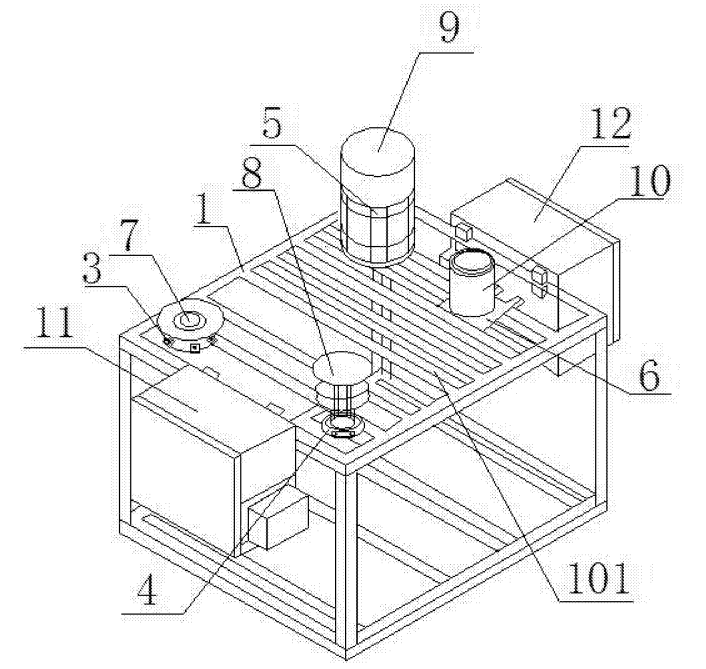
\includegraphics[width=\linewidth]{Recursos/Imagenes/ImagenesEstadoDelArte/CN206362955U.png}
	\end{minipage}\hfill
	\begin{minipage}{0.2\textwidth}
		\centering
		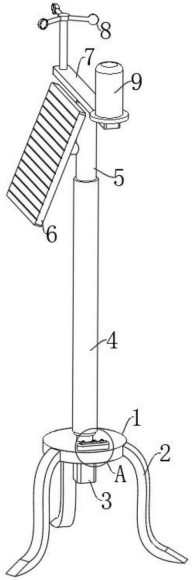
\includegraphics[width=\linewidth]{Recursos/Imagenes/ImagenesEstadoDelArte/CN222047271U-1.png}
	\end{minipage}
	\par\medskip
	
	\raggedright
	\footnotesize \textit{Nota.} Adaptado de \cite{CN206362955U} (izquierda) y \cite{CN222047271U} (derecha).
	\label{fig:CN206362955U&CN222047271U}
\end{figure}

    \item \textbf{Instrumentación electrónica para una estación meteorológica automática (MX 2018007917 A):} Esta patente define la arquitectura de instrumentación basada en microcontroladores para el registro de variables como irradiancia global, temperatura, humedad y viento. El sistema establece la lógica de procesamiento y almacenamiento de datos en módulos locales, sirviendo de base para la programación de registro de datos embebidos.
    
    \item \textbf{MeteoPV:} Este producto comercial, visto en la Figura \ref{fig:MeteoPV} (izquierda), es una plataforma de monitorización del recurso solar diseñada específicamente para aplicaciones fotovoltaicas distribuidas. Funciona como un adquisidor de datos compacto con interfaz web integrada que facilita la configuración de piranómetros inteligentes, celdas de referencia y sensores de temperatura posterior, transmitiendo la información mediante protocolos industriales como Modbus RTU y TCP/IP hacia sistemas SCADA.
    
    	\begin{figure}[H]
    	\captionsetup{justification=raggedright, singlelinecheck=false, labelsep=none}
    	
    	\caption[Imagen de controlador MeteoPV.]{} 
    	
    	\textit{Imagen de controlador MeteoPV.} \par\medskip
    	
    	\centering
    	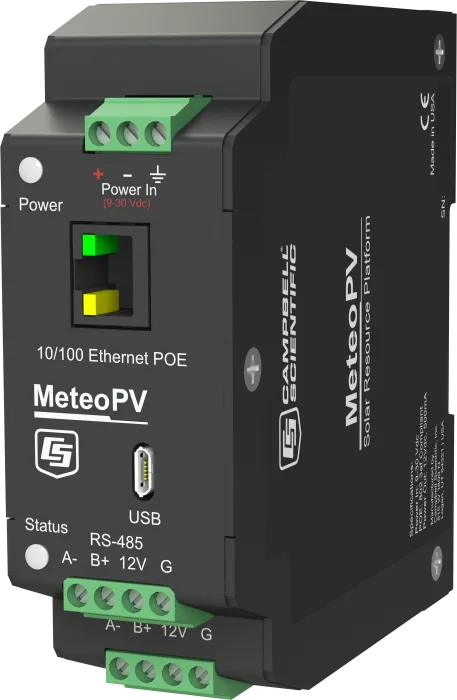
\includegraphics[width=0.3\textwidth]{Recursos/Imagenes/ImagenesEstadoDelArte/MeteoPV.png} \par\medskip
    	
    	\raggedright
    	\footnotesize \textit{Nota.} Adaptado de \cite{MeteoPV}.
    	\label{fig:MeteoPV}
    \end{figure}
\end{itemize}

\begin{center}
	\footnotesize
	\begin{xltabular}{\textwidth}{|p{3.5cm}|>{\raggedright\arraybackslash}X|>{\raggedright\arraybackslash}X|>{\raggedright\arraybackslash}X|}
		\caption{Análisis comparativo de Soluciones Parciales: Estaciones meteorológicas para plantas fotovoltaicas.}
		\label{tab:estado_arte_estaciones_pv} \\
		\hline
		\rowcolor[HTML]{D9E1F2} 
		\textbf{Referente} & \textbf{Principio de Funcionamiento} & \textbf{Aporte al Proyecto} & \textbf{Limitaciones} \\ \hline
		\endfirsthead
		
		\multicolumn{4}{c}%
		{{\bfseries Continuación de la \tablename\ \thetable{}}} \\
		\hline
		\rowcolor[HTML]{D9E1F2} 
		\textbf{Referente} & \textbf{Principio de Funcionamiento} & \textbf{Aporte al Proyecto} & \textbf{Limitaciones} \\ \hline
		\endhead
		
		\hline 
		\endfoot
		
		\hline
		\endlastfoot
		
		Estación meteorológica solar multi-elemento (CN 216243088 U) & Trípode adaptativo con sistema de anclajes de bloqueo por resorte para afianzarse al suelo. & Alternativa de fijación temporal para dar rigidez al mástil de medición frente a ráfagas de viento fuertes. & Naturaleza estática; su despliegue mecánico requiere que el vehículo se detenga por completo para realizar lecturas. \\ \hline
		Sistema de monitoreo de estación meteorológica para módulos fotovoltaicos (CN 206638837 U) & Marco estructural equipado con rieles y soportes móviles que ajustan la orientación de los piranómetros. & Principio geométrico aplicable para alinear los sensores con el ángulo de inclinación de los seguidores solares. & Sistema de ajuste manual; para el UGV requerirá integración con actuadores motorizados para operación autónoma. \\ \hline
		Estación meteorológica simple para monitoreo ambiental (CN 206362955 U) & Estructura estática compacta que integra en un solo marco sensores de radiación, viento, lluvia y temperatura. & Referencia para la distribución física de la suite de sensores a bordo de plataformas móviles, minimizando sombreados. & Diseño estático fijo que no permite la adaptación dinámica al ángulo de incidencia solar. \\ \hline
		Instrumentación electrónica para una estación meteorológica automática (MX 2018007917 A) & Arquitectura basada en microcontroladores para el registro de variables climáticas en módulos locales SD. & Establece la lógica de procesamiento y almacenamiento de datos para registradores de datos embebidos. & Sistema básico de registro sin capacidades de telemetría de largo alcance integradas. \\ \hline
		Micro estación meteorológica automática y retractable (CN 222047271 U) & Mástil de medición basado en un tubo telescópico extendido verticalmente por un motor eléctrico. & Permite elevar instrumentos para evadir las turbulencias y el polvo generado por el chasis móvil. & Elevar el mástil modifica el centro de gravedad del robot, lo que podría desestabilizarlo al transitar sobre pendientes. \\ \hline
		Plataforma MeteoPV & Datalogger comercial que concentra datos de sensores inteligentes y los transmite mediante Modbus RTU/TCP. & Prototipo comercial directo para la arquitectura de adquisición del UGV; asegura inmunidad ante el ruido de los motores. & Es un módulo pasivo diseñado para montaje estandarizado; requiere gestión de disipación térmica y no controla locomoción. \\ \hline
		
	\end{xltabular}
\end{center}
\subsubsection{Ajuste de orientación para sensores de irradiancia}

\begin{itemize}
	
	
    \item \textbf{Seguidor solar SOLYS2} Este producto, visto en la Figura \ref{fig:ZippZonen_Tracker&Radiometer} (derecha) es un seguidor solar de alta precisión que incluye un receptor GPS integrado para la configuración automática de las coordenadas geográficas y la hora. Su diseño permite un seguimiento exacto para orientar instrumentos de medición directa, eliminando la necesidad de ajustes manuales constantes o sincronización por computadora externa.
	
    
    \item \textbf{Kit de montaje para piranómetro con inclinación ajustable} Este producto, visto en la Figura \ref{fig:ZippZonen_Tracker&Radiometer}, trata de un soporte mecánico con escala graduada diseñado para montar piranómetros en ángulos de inclinación específicos de $0^{\circ}$ a $90^{\circ}$. Este kit permite igualar manualmente la inclinación de los sensores con la de los paneles fotovoltaicos fijos, asegurando que la irradiancia medida sea la misma que incide sobre la superficie de generación.
    
    
    \begin{figure}[H]
    	
    	\captionsetup{justification=raggedright, singlelinecheck=false, labelsep=none}
    	
    	\caption[Kit de montaje para piranómetro con inclinación ajustable de KIPP \& ZONEN.]{} 
    	
    	\textit{Fotos de módulo controlador MeteoPV y seguidor solar SOLYS2 de KIPP \& ZONEN.} \par\medskip
    	
    	\begin{minipage}{0.5\textwidth}
    		\centering
    		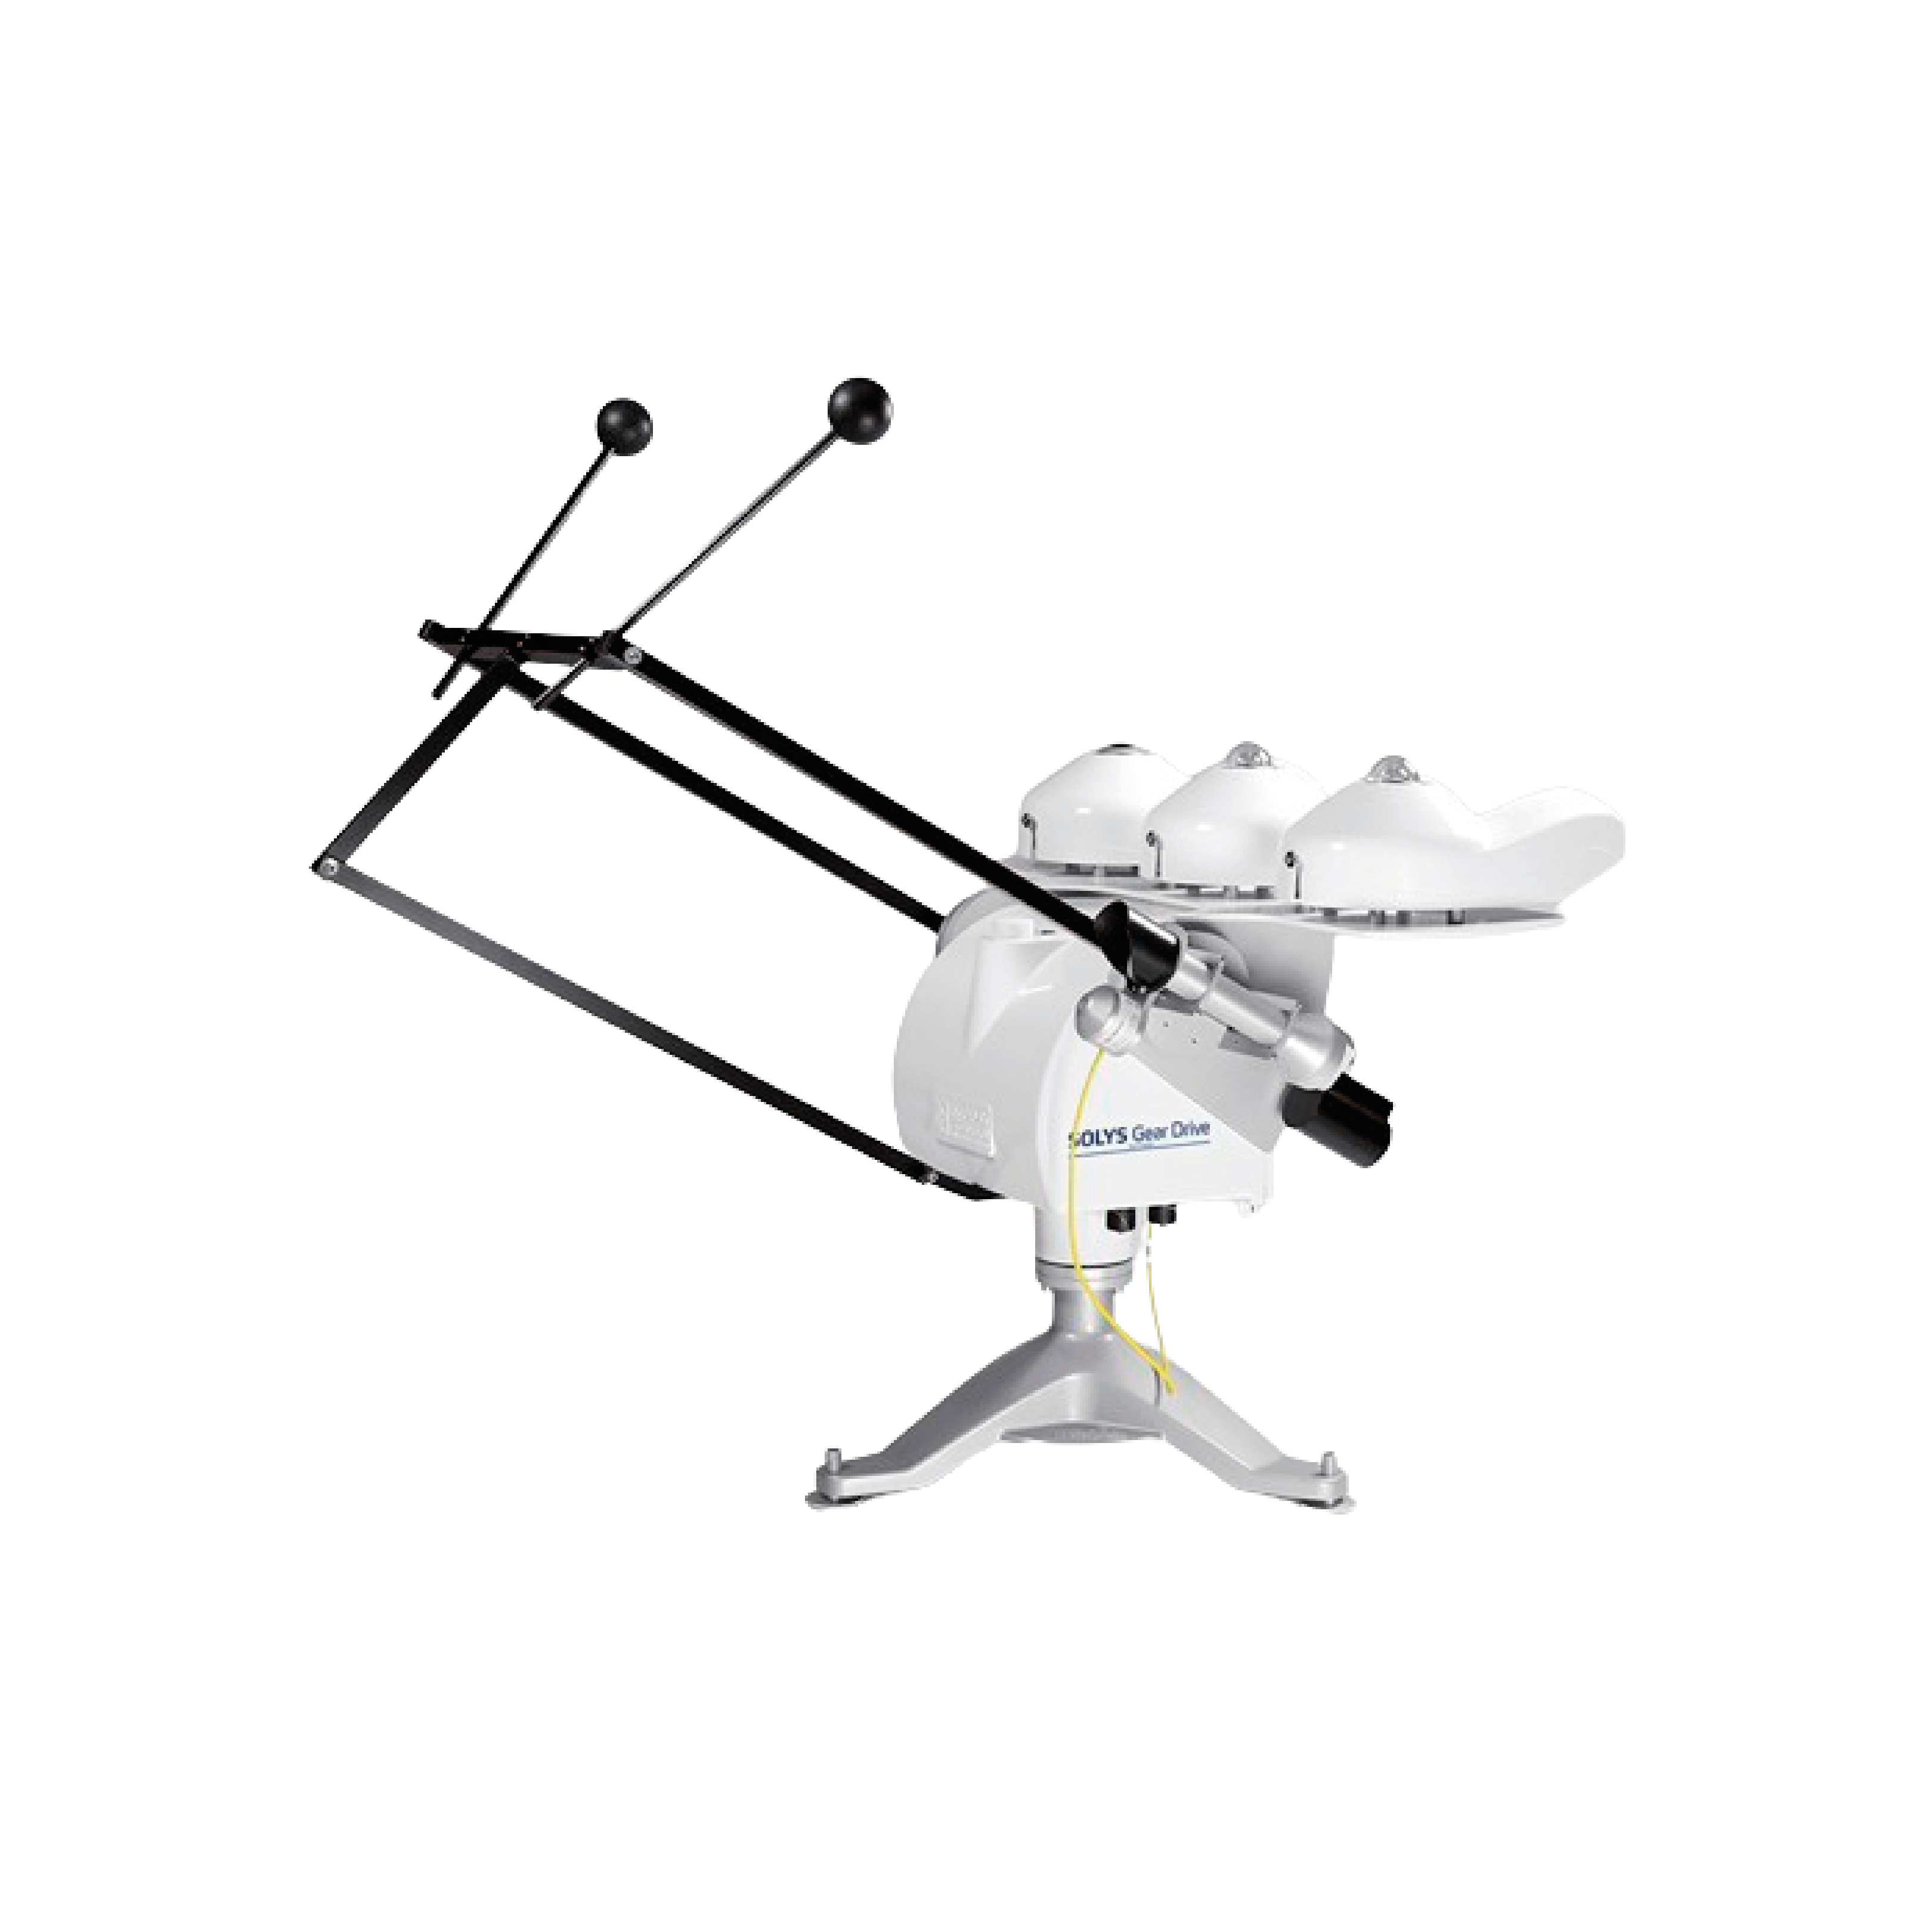
\includegraphics[width=\linewidth]{Recursos/Imagenes/ImagenesEstadoDelArte/KippZonen_SunTrackers.png}
    	\end{minipage}\hfill
    	\begin{minipage}{0.5\textwidth}
    		\centering
    		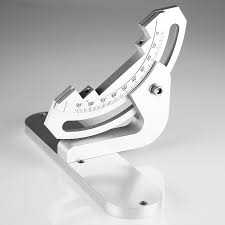
\includegraphics[width=\linewidth]{Recursos/Imagenes/ImagenesEstadoDelArte/KippZonen_Radiometer.jpg}
    	\end{minipage}
    	\par\medskip
    	
    	\raggedright
    	\footnotesize \textit{Nota.} Adaptado de \cite{KippZonen_SunTrackers} (izquierda) y \cite{KippZonen_Radiometer} (derecha).
    	\label{fig:ZippZonen_Tracker&Radiometer}
    \end{figure}
    
    
\end{itemize}
%
%
%%

\begin{table}[H]
	\centering
	\footnotesize
	\caption{Análisis comparativo de Soluciones Parciales: Ajuste de orientación para sensores de irradiancia.}
	\label{tab:estado_arte_ajuste_sensores}
	\begin{tabularx}{\textwidth}{|p{3.5cm}|>{\raggedright\arraybackslash}X|>{\raggedright\arraybackslash}X|>{\raggedright\arraybackslash}X|}
		\hline
		\rowcolor[HTML]{D9E1F2} 
		\textbf{Referente} & \textbf{Principio de Funcionamiento} & \textbf{Aporte al Proyecto} & \textbf{Limitaciones} \\ \hline
		Seguidor solar SOLYS2 & Seguidor solar automático con receptor GPS integrado para configuración autónoma de ubicación y tiempo. & Referencia para el seguimiento exacto de la trayectoria solar para instrumentos de medición directa. & Elevado peso y costo para ser integrado en una plataforma móvil de exploración dinámica. \\ \hline
		Kit de montaje para piranómetro con inclinación ajustable & Soporte mecánico con escala graduada para montaje de piranómetros en ángulos de $0^{\circ}$ a $90^{\circ}$. & Permite igualar manualmente la inclinación de los sensores con la de los paneles fotovoltaicos fijos (Plano POA). & Requiere intervención humana para el ajuste del ángulo de inclinación inicial. \\ \hline
	\end{tabularx}
\end{table}
%%
%
%


\subsubsection{Sistemas de comunicación para datos meteorológicos}
\begin{itemize}
    \item \textbf{Estación meteorológica avanzada IoT (SK 302020 A3):} Esta solución detalla un sistema meteorológico dividido en bloques funcionales, donde resalta un bloque avanzado de gestión y recuperación de baterías. Este esquema permite administrar la energía de los sensores de forma independiente a otros sistemas motrices, garantizando la continuidad de la toma de datos IoT incluso en condiciones de baja carga.
    
    \item \textbf{Sistema de monitoreo de plantación basado en LoRa (CN 208458788 U):} Este sistema utiliza la tecnología de comunicación inalámbrica LoRa para conectar múltiples nodos sensores, tanto móviles como fijos, con un gateway central. La arquitectura permite transmitir datos ambientales de irradiancia, viento y temperatura a largas distancias con bajo consumo energético, facilitando la supervisión remota a través de plataformas en la nube.
    
    \item \textbf{Método de posicionamiento para robots móviles (CN 116405876 A):} El método emplea módulos LoRa instalados en robots móviles que se comunican con gateways fijos distribuidos en el área de operación. Mediante el análisis de la intensidad de señal y el tiempo de llegada, el sistema permite determinar la ubicación precisa del vehículo en tiempo real y transmitir sus datos operativos hacia un servidor de control.
\end{itemize}

%
%
%%
\begin{table}[H]
	\centering
	\footnotesize
	\caption{Análisis comparativo de Soluciones Parciales: Sistemas de comunicación para datos meteorológicos.}
	\label{tab:estado_arte_comunicacion}
	\begin{tabularx}{\textwidth}{|p{3.5cm}|>{\raggedright\arraybackslash}X|>{\raggedright\arraybackslash}X|>{\raggedright\arraybackslash}X|}
		\hline
		\rowcolor[HTML]{D9E1F2} 
		\textbf{Referente} & \textbf{Principio de Funcionamiento} & \textbf{Aporte al Proyecto} & \textbf{Limitaciones} \\ \hline
		Estación meteorológica avanzada IoT (SK 302020 A3) & Sistema meteorológico IoT con un avanzado bloque de gestión y recuperación de baterías (BMS). & Permite administrar la energía de los sensores de forma independiente a otros sistemas motrices del vehículo. & No aborda aspectos de navegación o estabilidad mecánica requeridos para la movilidad en planta. \\ \hline
		Sistema de monitoreo de plantación basado en LoRa (CN 208458788 U) & Utiliza nodos sensores móviles y fijos conectados mediante red inalámbrica LoRa a un gateway central. & Permite la transmisión de datos a largas distancias con bajo consumo, ideal para supervisión remota en plantas extensas. & La latencia inherente a LoRa puede limitar la frecuencia de muestreo en inspecciones de alta velocidad. \\ \hline
		Método de posicionamiento para robots móviles (CN 116405876 A) & Emplea módulos LoRa para comunicación y cálculo de ubicación mediante intensidad de señal y tiempo de llegada. & Proporciona un método de localización en tiempo real para el seguimiento preciso de la ruta del vehículo. & Requiere la instalación de múltiples gateways distribuidos en el área operativa para garantizar precisión. \\ \hline
	\end{tabularx}
\end{table}

%%
%
%
El análisis de las soluciones tecnológicas actuales evidencia una brecha significativa en el sector para resolver el problema de los microclimas en topografías complejas. Por un lado, los vehículos terrestres desarrollados para la industria solar poseen sistemas de locomoción robustos capaces de superar desniveles, pero su instrumentación está limitada a inspecciones visuales o térmicas, lo cual es insuficiente para el mapeo climático dinámico exigido por la norma IEC 61724-1. Por otro lado, las estaciones meteorológicas móviles cuentan con los instrumentos correctos y sistemas de nivelación, pero carecen de la tracción y autonomía necesarias para transitar sobre pendientes extremas. En consecuencia, se justifica la necesidad de desarrollar el sistema mecatrónico propuesto en este proyecto: un robot híbrido que integre la posibilidad de locomoción con la implementación de instrumentación climática, capaz de nivelarse y operar autónomamente sobre los relieves de la instalación.


\end{document}